\documentclass{X:/Documents/Coding/Latex/myassignment}
%%Document info
\title{OFN Assignment 2}
\begin{document}
\includepdf{cover2}
\maketitle

\begin{enumerate}
\item Extremals for the functionals with $y(0) = 0, y(1) = 1$
\begin{enumerate}
	\item 
	\[F\{y\} = \int_0^1 \left(y^2 + y'^2 + 2ye^x\right) dx\]
	Euler-Lagrange:
	\[\odd{}x \left(\dd f{y'}\right)-\dd fy  =0\]
	\begin{align*}
		\dd fy = 2y + 2e^{x}\\
		\dd f{y'} = 2y'\\
		\odd{}x \left(\dd f{y'}\right) = 2y''
	\end{align*}
	Hence
	\begin{align*}
		2y'' - 2y - 2e^{x} = 0\\
		y'' - y - e^{x} = 0\\
		y''_{h} = y_{h}\\
		\implies y_{h} = c_1 e^{x} + c_2e^{-x}   
	\end{align*}
	Where $y_h$ is the homogeneous solution. Since the solution already contains $e^{x}$ try $xe^{x}$ for a particular solution
	\[y = c_1e^{x} + c_2e^{-x} + c_3 x e^{x}\]
	\[y'' = c_1 e^{x} + c_2 e^{-x} + c_3 (2e^{x} + xe^{x})\]
	\begin{align*}
		y'' - y - e^{x} &=c_1 e^{x} + c_2 e^{-x} + c_3 (2e^{x} + xe^{x}) -\left(c_1e^{x} + c_2e^{-x} + c_3 x e^{x}\right) - e^{x}\\
		0&= c_3\left(2e{x} + xe^{x} - xe^{x}\right) - e^{x}\\
		\implies  c_3 &= \frac12
	\end{align*}
	And hence
	\[y = c_1 e^{x} + c_2 e^{-x} + \frac12 xe^{x}\]
	\begin{align*}
		y(0) &= c_1 + c_2 = 0\\
		\implies c_2 &= -c_1\\
		y(1) &= c_1 e - c_1 e^{-1} + \frac12 e =1\\
		c_1(e-e^{-1}) &= 1 - \frac12 e\\
		c_1 &= \frac{1 - \frac12 e}{e - e^{-1}}
	\end{align*}
	So
	\[\boxed{y = \frac{1 - \frac12 e}{e - e^{-1}}\left(e^{x} - e^{-x}\right) + \frac12 xe^{x} }\]
	% \begin{align*}
	% 	F\{y\} &= \int_0^1 \left(y^2 + y'^2 + 2ye^x\right) dx\\
	% 	&=\int_0^1 \left( \left(c_1 e^{x} + c_2 e^{-x} + \frac12 xe^{x}\right)^2 + \left(c_1 e^{x} - c_2 e^{-x} +  e^{x} +\frac12 xe^{x}\right)^2 \right.\\
	% 	&+ \left.2e^{x}\left(c_1 e^{x} + c_2 e^{-x} + \frac12 xe^{x}\right) \right)dx\\\\
	% \end{align*}


	\item 
	\[F\{y\} = \int_0^1 (y^2 - y'^2 - 2y\sin x) dx\]
	\begin{align*}
		\dd fy &=2y - 2\sin x\\
		\dd f{y'} &= -2y'\\
		\odd{}x\left(\dd f {y'}\right) &= -2y''
	\end{align*}
	Euler-Lagrange gives
	\begin{align*}
		\odd{}x \left(\dd f{y'}\right)-\dd fy  =0\\
		-2y'' - 2y + 2\sin x = 0\\
		y'' + y - \sin x = 0
	\end{align*}
	The homogeneous solution:
	\[y_{h} = c_1\cos x + c_2 \sin x\]
	And particular solution can have $x\cos x$ and $x\sin x$ terms since $\cos x,\sin x $ are already in the homogeneous solution
	 \[y = c_1\cos x + c_2 \sin x + c_3 x\cos x +c_4 x\sin x \]
	 % \[y_p' = c_3 \cos x - c_3 x \sin x + c_4 \sin x + c_4x \cos x\]
	 \[y'' =-(c_1\cos x + c_2 \sin x) -2 c_3 \sin x - c_3x\cos x + 2c_4\cos x - c_4 x\sin x \]
	 \begin{align*}
	 	&y'' +y - \sin x =0\\
	 	&-2 c_3 \sin x - c_3x\cos x + 2c_4\cos x - c_4 x\sin x + c_3 x\cos x +c_4 x\sin x - \sin x = 0\\
	 	&-2 c_3 \sin x  + 2c_4\cos x - \sin x = 0\\
	 	&\implies c_4 = 0,\quad c_3 = -\frac12
	 \end{align*}
	 Hence
	 \[y = c_1 \cos x + c_2 \sin x - \frac12 x\cos x\]
	 Using the BCs:
	 \[y(0) = 0, y(1) =1\]

	 \begin{align*}
	 	y(0) = 0 \implies c_1 = 0\\
	 	y(1) = 1 \implies c_2\sin 1 - \frac12 \cos 1 = 1\\
	 	c_2 = \frac{1 + \frac12 \cos 1}{\sin 1}
	 \end{align*}
	 \[\boxed{ y = \frac{1 + \frac12 \cos 1}{\sin 1} \sin x - \frac12 x\cos x}\]
 	 
 	 % But I will keep it as $c_2$ for now for cleanliness sake.
	 % Plug into the functional
	 % \begin{align*}
	 % 	F\{y\} &= \int_0^1 (y^2 - y'^2 - 2y\sin x) dx\\
	 % 	&=\int_0^1 \left(c_2\sin x - \frac12 x\cos x\right)^2 - \left((c_2-\frac12)\cos x + \frac12 x\sin x\right)^2 - 2\sin x\left(c_2\sin x - \frac12 x\cos x\right) dx
	 % \end{align*}


\end{enumerate}

\item Consider
\[F\{y\} = \int_0^1 \left(\frac12 y'^2 + yy' + y' + y\right) dx, \quad y(0) = 0,\ y(1) = \frac32\]
\begin{enumerate}
	\item Determine the expression for $H$
	Since the functional doesn't depend on $x$
	\[H(y,y') = y' \dd f{y'} - f(y,y') = const\]
	\[\dd f{y'} = y' + y + 1\]
	\[
		H(y,y') = y'^2 +yy' + y'-\left(\frac12 y'^2 + yy' + y' + y\right) = const
	\]
	\item Derive $y(x)$ which is an extremal 

	\begin{align*}
 		y'^2 +yy' + y'-\left(\frac12 y'^2 + yy' + y' + y\right) = const	\\
 		y'^2 + 2y = k\\
 		y'^2 = k-2y\\
 		y' = \sqrt{k-2y}\\
 		\int \frac{dy}{\sqrt{k-2y}} = \int dx\\ 		
	\end{align*}
	Sub $ u = k-2y$, $dy = -\frac12 du$
	\begin{align*}
		\implies \int \frac{-1}{2\sqrt{u}} du = x-c\\
		-\sqrt{u} = x-c\\
		- \sqrt{k-2y} = x-c\\
		k-2y = (c-x)^2\\
		y = \frac{k - (c-x)^2}{2}
	\end{align*}
	And apply BCs:
	\[y(0) = 0 \implies k-c^2 = 0\]
	\[y(1) = \frac32 \implies k - (c-1)^2 = 3\]
	Subtract the two:
	\begin{align*}
		c^2 - (c-1)^2 = 3\\
		2c -1 = 3\\
		c = 2\\
		\implies k = 4
	\end{align*}
	\[\boxed{y = \frac{4 - (2-x)^2}{2}}\]
\end{enumerate}
\item 
\begin{equation}
	T\{y\} = \frac{1}{\sqrt{2g}} \int_{x_0}^{x_1} \sqrt{\frac{1 + y'^2}{y_0 -y}} dx	
	\label{eqn::brachfunct}
\end{equation}

With $y(x_0) = y_0$ and $y(x_1) = y_1$. We derived
\begin{equation}	
	x = x_0 + \kappa (\theta - \sin \theta), \quad y = y_0 - \kappa(1- \cos\theta),\quad 0\leq \theta \leq \theta_1	
	\label{eqn::brachsol}
\end{equation}
We must determine $\theta_1$ corresponding to $x=x_1$ and determine $\kappa$.
\begin{enumerate}
	\item Substitute the solution~\ref{eqn::brachsol} into the functional~\ref{eqn::brachfunct} and evaluate for an explicit form of $T$ (in terms of $\theta_1, \kappa, g$).

	Start with equation~\ref{eqn::brachsol}, and use the chain rule
	\begin{align*}
		\odd yx &= \frac{\odd y\theta}{\odd x\theta}\\
		&=	\frac{-\kappa\sin\theta}{\kappa - \kappa\cos\theta}\\
		&= \frac{\sin\theta}{\cos\theta -1}\\
		&= - \cot \frac{\theta}{2}
	\end{align*}
	\[\odd x\theta = \kappa (1-\cos\theta) \implies dx =\kappa (1-\cos\theta) d\theta\]
	\begin{align*}
		\theta_0 \implies x_0 &= x_0 + \kappa(\theta_0 - \sin\theta_0)\\
		\theta_0 = \sin\theta_0 \implies \theta_0 = 0
	\end{align*}
	We will ignore the $x_1$ case and just label it $\theta_1$ for now.

	\begin{align*}
		T\{y\} &= \frac{1}{\sqrt{2g}} \int_{x_0}^{x_1} \sqrt{\frac{1 + y'^2}{y_0 -y}} dx\\	
	 T\{\theta\}&= \frac{1}{\sqrt{2g}} \int_{\theta_0}^{\theta_1} \sqrt{\frac{1 + \cot^2\frac{\theta}{2}}{\kappa(1-\cos\theta)}} \kappa (1-\cos\theta) d\theta\\
	 &= \frac{\sqrt{\kappa}}{\sqrt{2g}} \int_{\theta_0}^{\theta_1} \sqrt{\left(1 + \cot^2\frac{\theta}{2}\right)(1-\cos\theta)} d\theta\\
	 &= \frac{\sqrt{\kappa}}{\sqrt{2g}} \int_{\theta_0}^{\theta_1} \sqrt{1 + \cot^2\frac{\theta}{2} - \cos\theta -\cos\theta \cot^2\frac{\theta}{2}} d\theta\\
	 &= \frac{\sqrt{\kappa}}{\sqrt{2g}} \int_{\theta_0}^{\theta_1} \sqrt{1 + \left(\frac{\sin\theta}{\cos\theta -1}\right)^2 - \cos\theta -\cos\theta \left(\frac{\sin\theta}{\cos\theta -1}\right)^2} d\theta\\
	 &= \frac{\sqrt{\kappa}}{\sqrt{2g}} \int_{\theta_0}^{\theta_1} \sqrt{\frac{(\cos\theta - 1)^2 + \sin^2\theta - \cos\theta (\cos\theta - 1)^2 - \cos\theta \sin^2\theta}{(\cos\theta - 1)^2}} d\theta\\
	 &= \frac{\sqrt{\kappa}}{\sqrt{2g}} \int_{\theta_0}^{\theta_1} \sqrt{\frac{\cos^2\theta -2\cos\theta + 1 + \sin^2\theta - \cos\theta (\cos^2\theta -2\cos\theta + 1) - \cos\theta \sin^2\theta}{(\cos\theta - 1)^2}} d\theta\\
	 &= \frac{\sqrt{\kappa}}{\sqrt{2g}} \int_{\theta_0}^{\theta_1} \sqrt{\frac{ -2\cos\theta + 2 - \cos\theta (-2\cos\theta + 1) - \cos\theta}{(\cos\theta - 1)^2}} d\theta\\
	 &= \frac{\sqrt{\kappa}}{\sqrt{2g}} \int_{\theta_0}^{\theta_1} \sqrt{\frac{2(1 -2\cos\theta + \cos^2\theta) }{(\cos\theta - 1)^2}} d\theta\\
	 &= \frac{\sqrt{\kappa}}{\sqrt{2g}} \int_{\theta_0}^{\theta_1} \sqrt{\frac{2(1-\cos\theta)^2 }{(\cos\theta - 1)^2}} d\theta\\
	 &= \frac{\sqrt{\kappa}}{\sqrt{2g}} \int_{\theta_0}^{\theta_1} \sqrt{2}d\theta\\
	T\{\theta\} &= \frac{\sqrt{\kappa}}{\sqrt{g}} \theta_1\\
	\end{align*}


	\item Assume $(x_0,y_0) = (0,2)$ and $(x_1,y_1) = (5,1)$ determine $\theta_1, \kappa$ for 3 different solution curves.

	$(x,y)$ solutions become
	\[	x = \kappa (\theta - \sin \theta), \quad y = 2- \kappa(1- \cos\theta),\quad 0\leq \theta \leq \theta_1	\]

	Solutions curves are those for which
	\begin{align*}
		5 = \kappa(\theta_1 - \sin\theta_1)\\
		1 = 2-\kappa(1-\cos\theta_1)
	\end{align*}
	\begin{align*}
		\kappa = \frac{5}{\theta_1 - \sin\theta_1}\\
		\implies 1 = 2 - \frac{5}{\theta_1 - \sin\theta_1}(1 - \cos\theta_1)\\
		\implies \theta_1 - \sin\theta = 5(1 - \cos\theta_1)\\
	\end{align*}
	Trivially $\theta = 0$ is a solution, but we will ignore this.
	Solutions are obtained guessed by observation (see fig~\ref{fig:int}) and then solved numerically using fzero, and are (to $4$ sf)
	\begin{figure}[h]
		\centering
		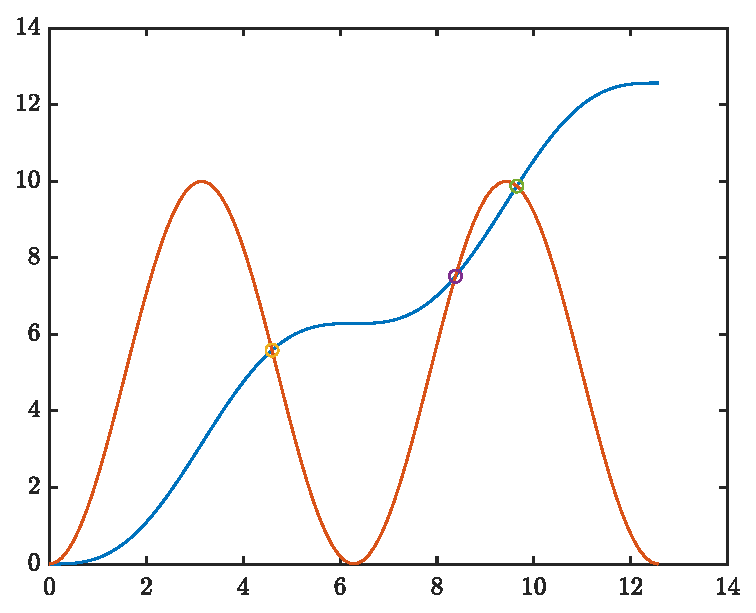
\includegraphics[width = 0.5\linewidth]{IntersectionPlot}
		\caption{Intersections corresponding to solutions for $\theta_1, \kappa$}
		\label{fig:int}
	\end{figure}
	\begin{align*}
		(\theta_1,\kappa)_1 &= (4.595,0.8948)\\
		(\theta_1,\kappa)_2 &= (8.382, 0.6651)
		(\theta_1,\kappa)_3 &= (9.650,0.5064)
	\end{align*}

	\item Take metres as the unit of length and $g=9.807m/s^2$, determine the value of $T$ for the three different solutions curves obtained in $(b)$. Give answers to four significant digits
	Corresponding to the combinations above:

	\begin{align*}
		(\theta_1,\kappa)_1 &= (4.595,0.8948) \implies T\{\theta\}_1 = 1.388\\
		(\theta_1,\kappa)_2 &= (8.382, 0.6651)\implies T\{\theta\}_2 = 2.183\\
		(\theta_1,\kappa)_3 &= (9.650,0.5064)\implies T\{\theta\}_3 = 2.193
	\end{align*}
	\item Plot the curves from $(b)$ and label them with the values of $T$ calculated in $(c)$.

	The plots are shown here. Figures~\ref{fig:figure1}, ~\ref{fig:figure2} and ~\ref{fig:figure3} show the three solutions.
	\begin{figure}[h]
		\centering
		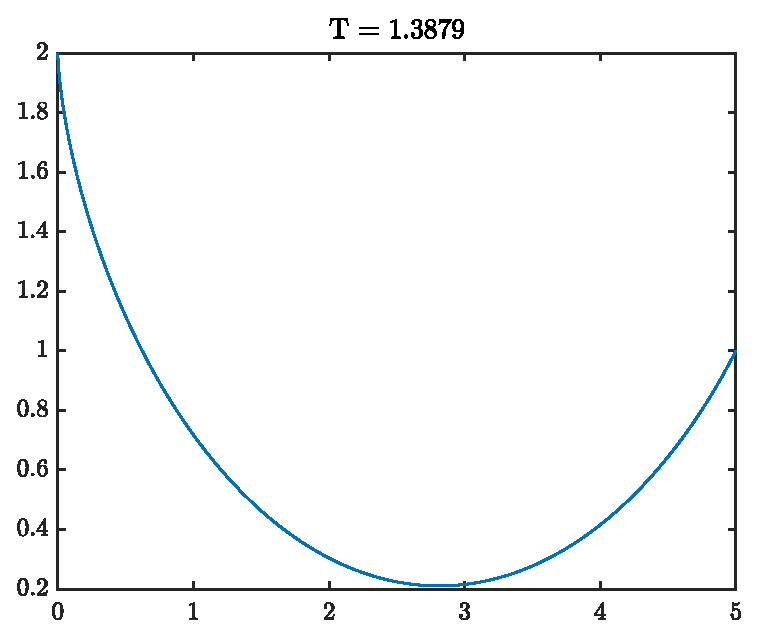
\includegraphics[width=0.5\linewidth]{Sol1}
		\caption{Solution plot for $(\theta_1,\kappa) = (4.595,0.8948)$}
		\label{fig:figure1}
	\end{figure}
	\begin{figure}[h]
		\centering
		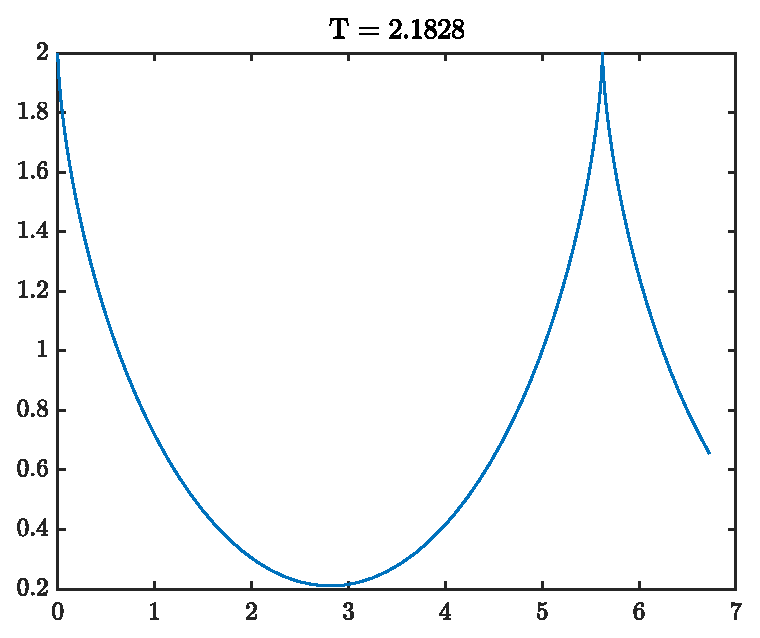
\includegraphics[width=0.5\linewidth]{Sol2}
		\caption{Solution plot for $(\theta_1,\kappa) =(8.382, 0.6651)$}
		\label{fig:figure2}
	\end{figure}
	\begin{figure}[h]
		\centering
		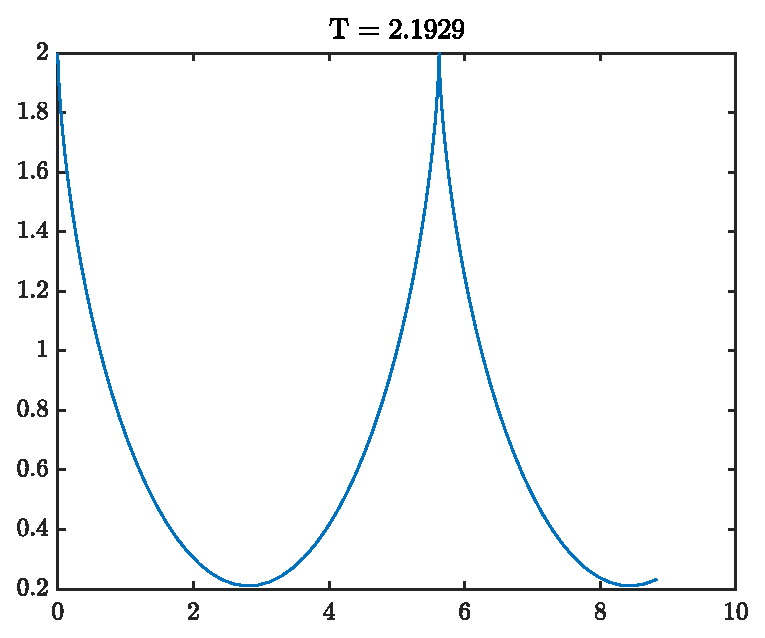
\includegraphics[width=0.5\linewidth]{Sol3}
		\caption{Solution plot for $(\theta_1,\kappa) =(9.650,0.5064)$}
		\label{fig:figure3}
	\end{figure}
	\clearpage
	The code used is below:
	\lstinputlisting{A2Code.m}
\end{enumerate}
\end{enumerate}

\end{document}